\documentclass[runningheads]{llncs}

\usepackage{ngerman}
\usepackage{graphicx}
\usepackage[utf8]{inputenc}
\usepackage{url}
\usepackage[square,sort,numbers]{natbib}
\usepackage{enumitem}

\urldef \urlEdgeContraction \url{https://commons.wikimedia.org/wiki/File:Edge_contraction.svg}
\urldef \urlPoligonSimplification \url{https://commons.wikimedia.org/wiki/File:Douglas_Peucker.png}

\urldef \urlDouglasPeckerAlg
\url{http://deacademic.com/dic.nsf/dewiki/34974}

\begin{document}

    \title{Vereinfachung von Oberflächen durch Nutzung von quadratischen Fehler-Matrizen}
    
    \titlerunning{Vereinfachung von polygonalen Oberflächen}
    
    \subtitle{1. Schreibaufgabe für Techniken des Wissenschaftlichen Arbeitens}
    
    \author{Nicolas Anton Gassen \\ Matrikel-Nr: 3230009 }
    
    \institute{Universität Bonn}
    
    \date{\today} 

\maketitle

\section{Einleitung}

Das Rendern von immer komplexer werdenden Objekten und deren Oberflächen wird trotz stetig besserer Hardware immer komplizierter und leistungsfordernder. Zudem müssen auch schwächere oder veraltete Geräte in der Lage sein aktuelle Programme die drei dimensionale Objekte nutzen mit akzeptabler Performance auszuführen. Um diesem Problem entgegen zu wirken kann man einen Algorithmus verwenden, welcher in der Lage ist übermäßig komplexe Oberflächen zu simplifizieren ohne einen übermäßigen Detailverlust mit sich zu bringen. \newline
Der vorgestellte Algorithmus greift diese Problematik vor allem in den Bereichen der Effizienz, Qualität und Allgemeinheit auf. Nach Eingabe eines Polygon Objektes berechnet das Programm mithilfe von Kantenkontraktion ein vereinfachtes Polygonmodell.\newline
Diese Methode besitzt eine enorm hohe Effizienz und ist deshalb in der Lage ein Modell mit 70.000 Polygonen, in nur etwa 15 Sekunden Zeitaufwand, auf nur 100 zu reduzieren[1]. Die Aproximierung der Oberfläche bleibt trotz geringerer Anzahl an Polygonen nahe an der originalen Form und bleibt deshalb qualitativ erhalten.\newline 
Andere Algorithmen die sich mit der gegebenen Problematik befassen sind meist nicht in der Lage disjunkte Objekte aufgrund fehlender Polygonverbindungen sinnvoll zu Vereinfachen.\newline
Durch Gruppierung von Kanten können fehlende Verbindungen zwischen Polygonen ergänzt werden. Dies bringt die Möglichkeit einer weitaus stärkeren und genaueren Simplifizierung so lange die Netztstruktur des gegebenen Objektes nicht zu essentiell ist.

    \subsection{Stand der Forschung}
        Ältere Algorithmen mit demselben Ziel haben das Problem das disjunkte Polygone nicht vereint werden und daher nur eine limitierte Menge an Genauigkeit und Vereinfachung bei Oberflächen erzielt werden kann, welche Polygone enthalten die zwar nah bei einander sind aber keine direkte Verbindung besitzen. Mithilfe des Prozesses der Kantenkontraktion kann die Anzahl an Polygonen weiter reduziert werden.

\section{Vereinfachung der Polygonmodelle}

    \subsection{Kantenbegradigung}
    Um die Anzahl der benötigten Polygone zu reduzieren werden alle Kanten begradigt indem überflüssige Punkte entfernt werden. 
    Die Oberfläche wird hier nur auf die nötigsten Punkte reduziert welche anschließend durch neue Verbindungen wieder zu Polygonen erweitert werden[2].\newline
    Der Prozess versucht neue Linien zu ziehen ohne die Form zu weit zu verändern und ist daher vergleichbar mit dem Douglas Peucker Algorithmus[5]. 
    Dieser ist in der Lage unter einem gegebenen Toleranzwert die Anzahl der benötigten Punkte unter Berücksichtigung des Toleranzwertes zu verringern.
    Anstelle von simplen Linien auf einer zwei dimensionalen Ebene (siehe Abbildung \ref{fig:Polygonsimplifizierung}) werden drei dimensionale Vektoren verwendet.\newline
    
    \begin{figure}[ht]
	\centering
	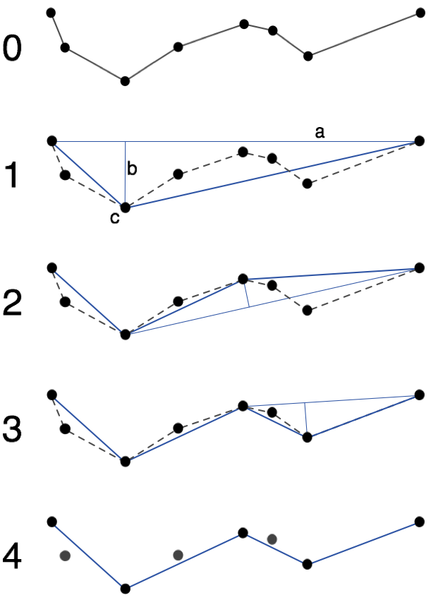
\includegraphics[width=0.25\textwidth]{Polygonsimplifizierung.png}
	\caption{Polygonsimplifizierung [3].}
	\label{fig:Polygonsimplifizierung}
\end{figure}

\subsection{Schließen von Lücken zwischen Polygonen}
    Viele Algorithmen haben Probleme mit Objekten bei denen die Form bei der Vereinfachung wichtiger ist als der Beibehalt der exakten Topologie des Objektes [1]. 
    Dort kann es passieren, dass wenn nahe liegende Polygone ohne direkte Verbindung nicht verbunden werden bei der Vereinfachung Löcher entstehen. Der gegebene Algorithmus ist jedoch in der Lage durch Gruppierung und Verkürzung nahe Liegender Punkte die Lücken zu schließen (Siehe Abbildung \ref{fig:KantenKontraktion}). \newline
    Die Kontraktion funktioniert wie folgt:\newline
    ''A pair contraction, which we will
    write ($v$, $u$ ) to $w$, moves the vertices $v$ and u to the new position
    $w$, connects all their incident edges to $v$, and deletes the vertex $u$. 
    Subsequently, any edges or faces which have become degenerate are removed.'' [1] (Vergleiche Abbildung \ref{fig:KantenKontraktion}).
    
    \begin{figure}[ht]
	\centering
	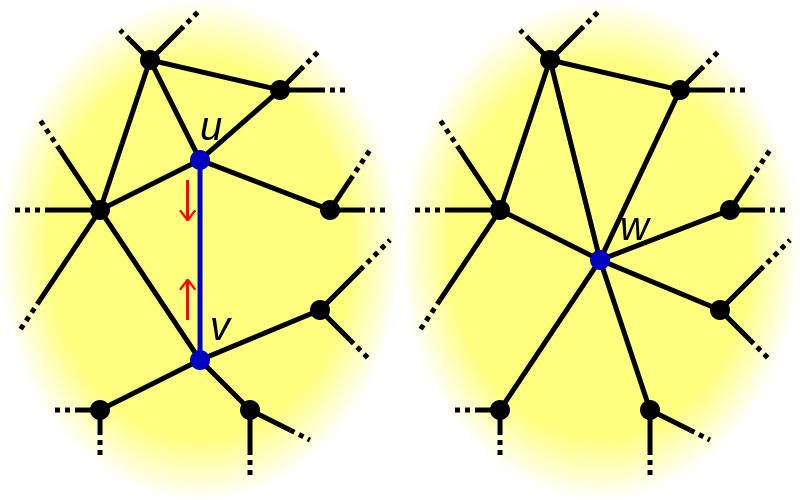
\includegraphics[width=0.6\textwidth]{KantenKontraktion.png}
	\caption{Kantenkontraktion [4].}
	\label{fig:KantenKontraktion}
    \end{figure}

\noindent

\section{Algorithmus}
\subsection{Auswahl von validen Paaren}
    Um Lücken zu schließen müssen Vektorpaare gebildet werden für die eine Verneinung Sinnvoll sind. Für die Auswahl sind zwei Punkte von hoher Wichtigkeit:
    \begin{enumerate}
    \item[``1.] ($v1$, $v2$ ) is an edge, or
    \item[2.] \textbar \textbar $v1$ - $v2$ \textbar \textbar \textless $t$, where $t$ is a threshold parameter'' [1].
    \end{enumerate}

\subsection{Berechnung der Fehlermatrizen}
    Um letzten Endes zu entscheiden ob ein Paar kontaktiert werden kann muss der relative Fehler der durch die Kontraktion entsteht berechnet und evaluiert werden ob der Fehler in der erlaubten Abweichung liegt.\newline
    Da der Fehler quadratisch zu beschreiben ist kann man ihn in einer simple lineare Funktion beschreiben. Wenn man Funktion \ref{eq:1} auflöst erhält man den geringsten Fehler und kann mit dem neu gebildeten Vektor $u$ und $v$ zu $w$ vereinen (Vergleiche Abbildung \ref{fig:KantenKontraktion}).
    
    \begin{equation} \label{eq:1}
    \frac{\partial \delta}{\partial x} = \frac{\partial \delta}{\partial y} = \frac{\partial \delta}{\partial z} = 0 
    \end{equation}
    Die Fehlermatrix ist äquivalent zu Funktion \ref{eq:1}:
    $\left[ \begin{array}{rrrr}
    q11 & q12 & q13 & q14 \\
    q21 & q22 & q23 & q24 \\
    q31 & q32 & q33 & q34 \\
    0 & 0 & 0 & 1 \\
    \end{array}\right] \overline{v} = 
    \left[ \begin{array}{r}
    0\\
    0\\
    0\\
    1 \\
    \end{array}\right] $\newline
    \subsection{Durchführung}
    Zu Beginn werden für alle Ecken des Objektes entsprechende 4x4 Matrizen bestimmt von diesen dann alle validen Paare ausgewählt werden. Anschließend wird zu jedem Paar eine Fehlermatrix ausgerechnet und der minimale Fehlervektor $\overline{v}$ entnommen. Die Beträge aller $\overline{v}$ werden in eine Liste geschrieben wobei die Paare mit dem geringeren Fehler (Betrag des Fehlervektors) weiter oben in der Liste sind.\newline
    Erst jetzt wird die Kontraktion ausgeführt: Das Paar ($v1, v2$) mit dem geringsten Fehler wird der Liste entnommen und zu $v$ kontraktiert. Weil $v2$ entfernt wurde müssen nur alle Paare in der Liste die $v1$ enthalten neue Berechnet werden.\newline
    Es wird so lange kontraktiert bis die gewünschte Menge an Vereinfachung erreicht wird oder weniger als 3 Elemente (ein Polygon) übrig bleiben. \newline
    Eine solche Vereinfachung ist in Abbildung \ref{fig:Vereinfachung} zu sehen.
    
    \begin{figure}[ht]
	\centering
	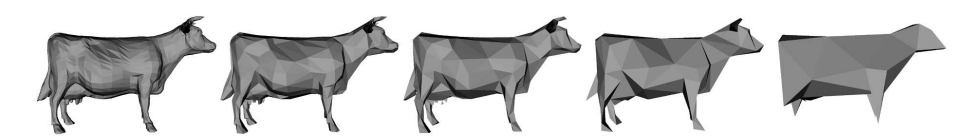
\includegraphics[width=1\textwidth]{Vereinfachung.png}
	\caption{Vereinfachung eines Objektes von 5.804 Oberflächen zu 994, 532, 248, und 64. [6].}
	\label{fig:Vereinfachung}
    \end{figure}

\section{Schlusswort}
Vereinfachungen unter der Nutzung von diesem Algorithmus haben einen minimalen Fehler und sind in der Lage auch Objekte mit fehlenden Polygonverbindungen in einer angemessenen Qualität auf eine geringe Polygonanzahl zu bekommen.\newline
Frühere Algorithmen haben häufig Probleme bei einer Vereinfachung von Objekten mit vielen heraus stehenden Details. Diese erhalten nach dem Durchlauf häufig Löcher oder behalten die Details nicht bei. \newline
Durch die beschriebene Kontraktionsmethode ist dies allerdings kein Problem und es kann durch den beschriebenen Algorithmus deutlich stärker und akkurater Simplifiziert werden ohne einen zu starken relativen Fehler, im Vergleich zu früheren Algorithmen, mit sich zu ziehen.\newline
Unter anderem wird der ungefähren prozentualen Fehler der Vereinfachung ausgelesen ohne einen direkten Vergleich des Eingangs- und Ausgabemodells zu tätigen.
Der Algorithmus kann soweit das Eingabeobjekt aus Polygonen besteht jedes Objekt bis auf die gewünschte Menge an Oberflächen reduzieren.\newline
Die Laufzeit ist selbst für komplexe Objekte sehr gering.\newline
Das Modell der Kuh in Abbildung \ref{fig:Vereinfachung} kann zum Beispiel in etwa 910ms (220ms Paarbildung und Matrizenberechnung und 690ms Kontraktierung) auf 10 Oberflächen reduziert werden [1].\newline
Zusammenfassend kann man behaupten, dass der Algorithmus Allgemein, Akkurat und Schnell ist. Was ihn für die Nutzung zur Vereinfachung von Objekten jeglicher Art sinnvoll macht.

\begin{thebibliography}{5}

\bibitem{1}
Michael Garland und Paul S. Heckbert; Carnegie Mellon University, ''Surface simplification using quadric error metrics'' 
ACM Press/Addison-Wesley Publishing Co. 1997

\bibitem{2}
Alan D. Kalvin und Russell H. Taylor, ''Superfaces:polygonal
mesh simplification with bounded error'', IEEE Computer
Graphics and Appl., 16(3), May 1996

\bibitem{3}
Darstellung einer Polygonsimplifizierung, \urlPoligonSimplification, abgerufen am 23.10.2018.

\bibitem{4}
Darstellung einer Kantenkontraktion, \urlEdgeContraction, abgerufen am 24.10.2018.

\bibitem{5}
douglas peucker algorithm, \urlDouglasPeckerAlg, abgerufen am 24.10.2018

\bibitem{6}
Bild entnommen aus: Michael Garland und Paul S. Heckbert; Carnegie Mellon University, ''Surface simplification using quadric error metrics'' 
ACM Press/Addison-Wesley Publishing Co. 1997
\end{thebibliography}

\end{document}